\chapter{Previous work}\thispagestyle{empty}
\par{
    This chapter gives an overview of the previous work in two fields combined in this project.
    First there is the application of \Gls{ai}\footnote{For a brief introduction of \Gls{ai} and \Gls{machinevision} itself, please consult chapter \ref{sec:ai_and_ml}.} 
    in medical applications, specifically for \Gls{machinevision} problems.
    Then, there is the active area of research of \Gls{weaklysupervisedl} machine learning both for medical and for non-medical applications.
}

\section{Machine vision for medical applications\label{sec:MachineVisionMedical}}

\par{
    For segmentation tasks, the U-net architecture\cite{Ronneberger2015} is widely used\footnote{The U-net architecture was developed specifically for biomedical applications.}. 
    This architecture can be represented by a characteristic U-shape (see figure \ref{fig:unet}), as the name indicates.
    This architecture is based on a \textit{contracting} resolution path followed by an \textit{expanding} path. 
    The contracting path refers to the resolution reduction in each step. 
    These steps consist of two convolution layers, of which the result is used in two ways. 
    First, the convolution layer result is \textit{down-sampled} (the layer dimension is reduced) with a max-pooling layer.
    In each contracting step, the number of feature channels is increased, allowing the network to propagate context information and produce feature maps with more high-level features.
    Second, this convolution layer result is concatenated with the corresponding feature maps in the expanding path.
    These expanding steps consist of inverse convolution layers, expanding the layer dimensions. To some extent, the expanding path is symmetric to the contracting path, giving the network its U-shape. 
    The connections where the convolution layer results of the contracting path are concatenated to the corresponding layers in the expanding path are called the \textit{skip connections}.
    Through these connections, the network can propagate information efficiently over different resolution levels\footnote{Skip connections have proven efficient tools to decrease problems such as gradient vanishing.}.
    The 2-dimensional network developed in \cite{Ronneberger2015} was first adapted for three-dimensional problems in \cite{Cicek2016}.
}
\begin{SCfigure}[][htb]
    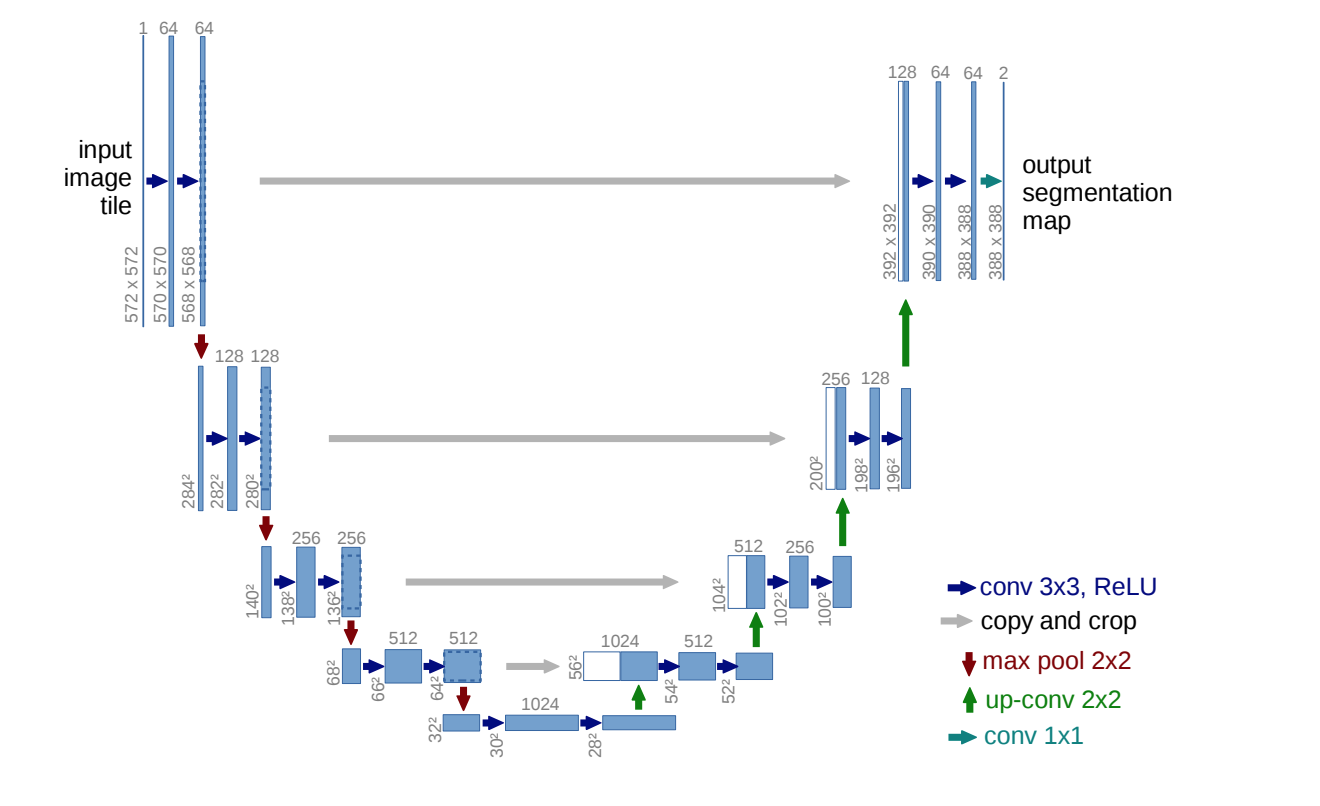
\includegraphics[width=10cm]{/home/thesis/images/UNet_Ronneberger.png}
    \caption{U-Net architecture, as illustrated in \cite{Ronneberger2015}. 
    Each blue box represents a multi-channel feature-map. 
    The number of channels is indicated above the box, the $x \times y$ dimensions are indicated at the bottom left.
    The gray arrows indicate the feature maps in the contracting path are copied and concatenated to the feature maps of the expanding path.}
    \label{fig:unet}
\end{SCfigure}
\par{
    Various segmentation architectures are based on similar ideas: first, a high-level feature map is created in a contracting path. 
    This feature maps is sometimes called the image \textit{encoding}. 
    Subsequently, this feature map is \textit{decoded} in an expanding path to form the segmentation mask. 
}


\subsection{Automated segmentation of the human spine}
\par{
    Multiple researchers have build systems for the automated segmentation of the human spine.
    Historically, this was done with techniques based on the calculation of mathematical and geometrical features of vertebrae. 
    For example in \cite{Klinder2008}, a model registration approach is used to segment a set of 10 \acrshort{ct} images.
    A parametric geometrical model of a spine is optimized to fit the scan geometry as good as possible.
    These techniques showed to suffer from difficulties to generalize
    \footnote{Before the general introduction of deep learning, limits to the model's capability to generalize were observed in many different applications.
    This could be improved with deep learning networks, at the cost of requiring higher data volumes, higher data variability and often higher computation cost.
    Simply put, the higher number of model degrees of freedom, combined with the ability to work without human encoded features, allows a better representation of the complex and variable reality.}. 
    When the scan geometry does not match closely to an ideal spine, for example, when a patient has severe scoliosis, this approach runs into problems.
    Before the general introduction of deep learning networks, techniques such as Viola-Jones detectors were used, such as in \cite{Zukic2014}. 
    A project of which the dataset is discussed on page \pageref{sec:DataUSiegen}.
}
\par{
    Deep learning models were developed for the problem \cite{Sekuboyina2017, Janssens2018, Chuang2019, Lessmann2018}.
    The model in \cite{Sekuboyina2017}\footnote{This model is developed on the xVertSeg dataset, which is one of the datasets used in this work. It is described starting on page \pageref{sec:xVertSeg}.} 
    uses a multi-step approach. First, the \acrfull{roi} (the lumbar region) is selected using a multilayer perceptron evaluated on the response of a Canny Edge filter.
    This \acrshort{roi} is then sliced (sagittal) and crops ($270mm \times 270mm$\footnote{The article also mentions $27mm \times 27mm$, which seems to be a typo.}) are segmented with a 2D U-net. 
    The resulting masks are improved with a morphological closing filter. 
    In \cite{Janssens2018}, a similar 2 step approach is used. Here, the author chose to use a 3D U-net to evaluate patches from the \acrshort{roi} instead of a 2D U-net.
}
\par{
    An interesting approach to the problem is published in \cite{Lessmann2018, Chuang2019} by Lessman and Chuang. 
    The approach presented in this work makes use of the available prior anatomical knowledge of the human spine: 
    the vertebrae are located right next to each other and always occur in the same, known order.  
    The basis of the network in \cite{Lessmann2018} is an extended 3D U-Net, combined with an elaborate inference scheme.
    In \cite{Chuang2019}, this network was improved to reduce the memory required and the complexity of the inference scheme.
}
\par{
    In figure \ref{fig:lessmann_inference}, the inference scheme used in \cite{Lessmann2018} is illustrated.
    This approach is based on the anatomical knowledge that vertebrae occur in order, right next to each other.
    The network, illustrated in figure \ref{fig:chuang_architecture} in the version as presented in \cite{Chuang2019}, 
    performs instance segmentation of the scan by sequentially evaluating the model on 3-dimensional patches of the scan. 
    These patches have dimensions $180mm \times 180mm \times 180mm$ and can thus contain a complete vertebra and meaningful parts of one or two adjacent vertebrae.
    The model is trained based on an image patch combined with a memory patch. This memory patch contains the voxels of the vertebrae that were already segmented in the sequential procedure.
    The network is trained to segment only the consecutive vertebra in sequence.
    For inference, the procedure evaluates patches from the scan border until a (partial) vertebra is discovered and segmented.
    After storing this first segmented vertebra in the memory patch, the next vertebra is segmented from a patch that is centred on the previous vertebra and shifted down
    \footnote{The procedure works both for sampling up-down and down-up. Here, I stay with the procedure illustrated in figure \ref{fig:lessmann_inference}.}.
    Following this procedure, the vertebrae are segmented one by one.
    This procedure was developed on a collection of 103 medical images of the human spine, including the xVertSeg dataset (discussed on \pageref{sec:xVertSeg}). 
    To improve the segmentation result, a \textit{soft false positive} and \textit{soft false negative} loss is added to the cross-entropy loss, where the voxels are weighted by the inverse of the distance to the segment border. 
    These terms increase the loss specifically for those voxels close to the edge of a vertebra.
}
\begin{SCfigure}[][htb]
    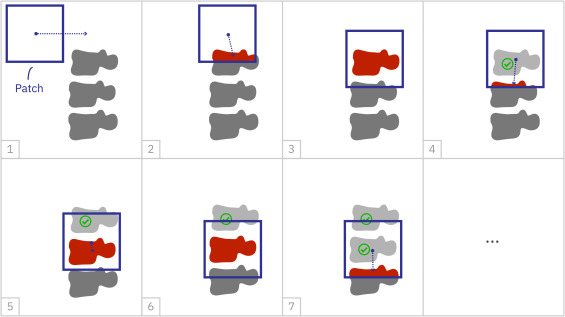
\includegraphics[width=10cm]{/home/thesis/images/Lessman_inference.jpg}
    \caption{Illustration of the inference scheme used in \cite{Lessmann2018} (image taken from same). }
    \label{fig:lessmann_inference}
\end{SCfigure}
\par{
    In \cite{Chuang2019}, some improvements to this procedure were introduced.
    The model is rendered less memory-intensive bypassing the feature maps in the skip-connections after unspooling instead of directly.
    A method is developed to improve finding the starting point of the sequential segmentation procedure by evaluating only the patches where a high bone density is observed.
    The network is trained to output 3 values:
    \begin{description}
        \item[classification $C$]: A classification result of the segmented vertebra (in the specific evaluation step).
        \item[instance segmentation mask $S_1$]: A segmentation mask that indicates to what vertebra instance every voxel in the patch belongs. 
        \item[Semantic segmentation mask $S_2$]: A binary segmentation mask that indicates whether a voxel belongs to a vertebra or to the background class.
    \end{description}
    To some extent, these three outputs seem redundant. 
    Labelling the individual vertebrae is a challenging task since there is a very high geometric correlation between vertebrae.
    Thus, a combination of different estimations is intended to procedure more reliable labelling.
}
\begin{SCfigure}[][htb]
    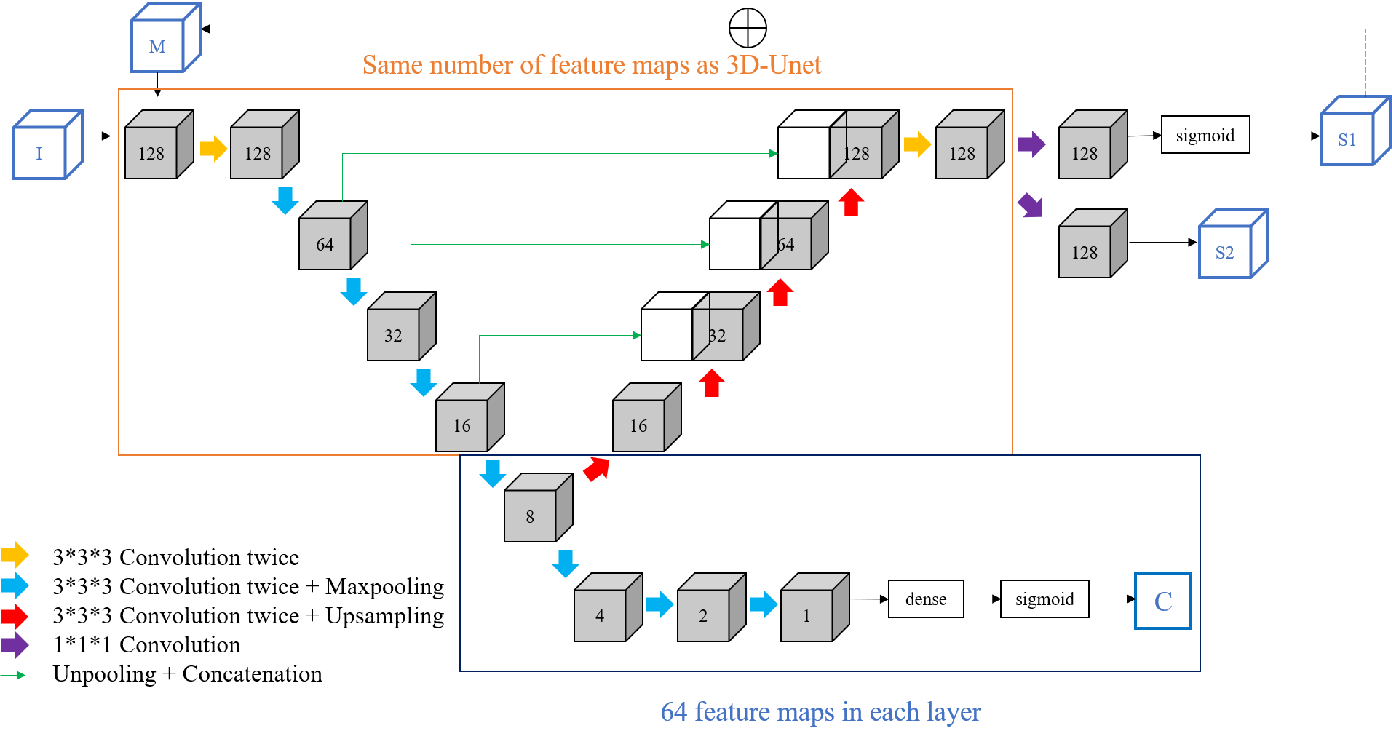
\includegraphics[width=10cm]{/home/thesis/images/Chuang_architecture.png}
    \caption{Extended U-Net architecture. Image from \cite{Chuang2019}.
    This network has }
    \label{fig:chuang_architecture}
\end{SCfigure}

%\todo[inline]{other authors, approaches --> priors used, metrics used, datasets used}


\section{Weakly supervised segmentation\label{sec:PreviousWork_weaklySupervised}}
\par{
    The subject of \Gls{weaklysupervisedl} is broad.
    Researchers devised various ideas to decrease the labelling cost by leveraging weak labels to infer strong results.
    Chapter \ref{sec:weak_supervision} discribes a number of different annotation types.
}
\subsection{General overview of techniques and approaches}
\par{
    To solve the weakly supervised problem, different authors\cite{Laradji2019,Laradji2019a, Ahn2019,McEver2020} share the same high-level technique to work in a two-step procedure, first estimating point guided pseudo-masks, then training a network based on these pseudo-masks.
    The construction of these pseudo masks is performed differently.
}
\par{
    Given an image-level class label, the Grad-\Gls{caml} \cite{Selvaraju2020} allows to identify the picture regions responsible for a classification result.
    The basic idea is to trace back the gradient to identify pixels for which changing the pixel value would change the model classification output.
    The pixels that incite the model to predict a certain class correspond to images of this class. In \cite{Selvaraju2020} these are used as pseudo masks to train a segmentation network, only based on image-level labels.
    Ahn et al. \cite{Ahn2019} combines the pseudo masks generated with CAM with an inter-pixel relation map.
    Since the mask generated by using CAM cannot distinguish between different instances of the same semantic class, it is not suitable for generating instance (pseudo) masks.
    In \cite{Ahn2019}, these masks are combination with (semantic class agnostic) inter-pixel relation maps that can make a difference between different instances.
    This inter-pixel relation map is trained by encouraging the model to identify an instance boundary between pixels with different class affinity and by identifying a limited number of instance centroids.
    Other pseudo mask generation methods exist, for example methods based on partial image occlusion or erasing\cite{Wei2017}.
    In this approach, image regions associated with different classes are identified by training an adversarial network to erase regions of the image to change the classification output.
    The idea is identical to the approach based on CAM: detect the regions of the picture responsible for the classification result.
}
\par{
    The techniques mentioned above make use of image level annotation.
    This work is based on weak labels containing a higher level of information: point annotation.
    The rationale behind point annotation is that when an expert is required to label the images, optimal use needs to be made of the expert's time.
    Based on estimations \cite{Bearman2015} the time consumption of point annotation and image level annotation is small, yet the information quality is higher (see also chapter \ref{sec:weak_supervision}).
    An expert does not need significantly more time to click on an object compared to providing an image label\footnote{
        It should be noted that point annotation refers to \textit{random} point annotation. Some authors \cite{Maninis2018} use \textit{extreme} point annotation. 
        Where the expert is requested to indicate points at the edge of the segment region.
    }, yet the point provides valuable localization information.
    In \cite{McEver2020}, the case is even made that for large and dense images, point annotations could even help the expert to keep track of the already labelled objects.
    By using the annotation points, in a technique called \acrfull{pcam}, the authors of \cite{McEver2020} can improve the quality of the class affinity estimation compared to the regular \Gls{caml} technique (using the PASCAL VOC 2012 dataset).
    The obtained affinity maps are subsequently used as \textit{pseudo} label maps to train a network (ResNet50). 
    The author reports an improved performance of the model trained on \textit{pseudo} labels compared to the performance metric calculated for those pseudo labels.
}

\subsection{Weakly supervised segmentation for Medical applications}
\par{
    dr. I. Laradji developed several methods to make use of point supervised data for segmentation tasks.
    First, LC-FCN is introduced: \acrfull{fcn} with a \acrfull{lc} as optimization loss.
    This technique was introduced by I. Laradji et al. in \cite{Laradji2018} for the training of an automated instance counting network on point-supervised data.
    Later it is applied in \cite{Laradji2020} as the Location branch of the WISE network.
    Contrary to other \Gls{weaklysupervisedl} projects, the authors focus on multi-class, multi-instance problems for which CAM-based solutions are less suitable.
    This method, illustrated in figure \ref{fig:Laradji_WISE}, consists of two branches from the same backbone: the Embedding branch and the Localization branch.
    The Embedding branch is trained with a pre-trained class-agnostic object proposal method. 
    This network (FCN8) is pre-trained to output similar embeddings for pixels that belong to the same class.
    The output of the network is thus an Embedding mask for each pixel of the image. 
    This network is trained to deliver different embeddings for different object instances with a binary cross-entropy function on the squared exponential kernel difference of the embeddings
    \footnote{With $E_i$ and $E_j$ the embeddings for points $i$ and $j$ and $\mathcal{I}$ the collection of labelled points.}:
}
\begin{eqnarray*}
    S(i,j) &=& \exp \left( \frac{||E_i-E_j||^2}{2d} \right)\\
    \mathcal{L}_E &=& - \sum_{(i,j)\in \mathcal{I}} [  \mathbf{I}(y_i=y_j) log(S(i,j)) \\ &+& \mathbf{I}(y_i\neq y_j) log(1-S(i,j))  ]
\end{eqnarray*}
\par{
    The second part of the WISE network is the Localization branch. 
    This branch aims to predict small \textit{blobs} at the centre of each object.
    These blobs are too small to serve as masks on their own, but they can be combined with the E-branch result to provide segmentation masks.
}
\begin{SCfigure}[][htb]
    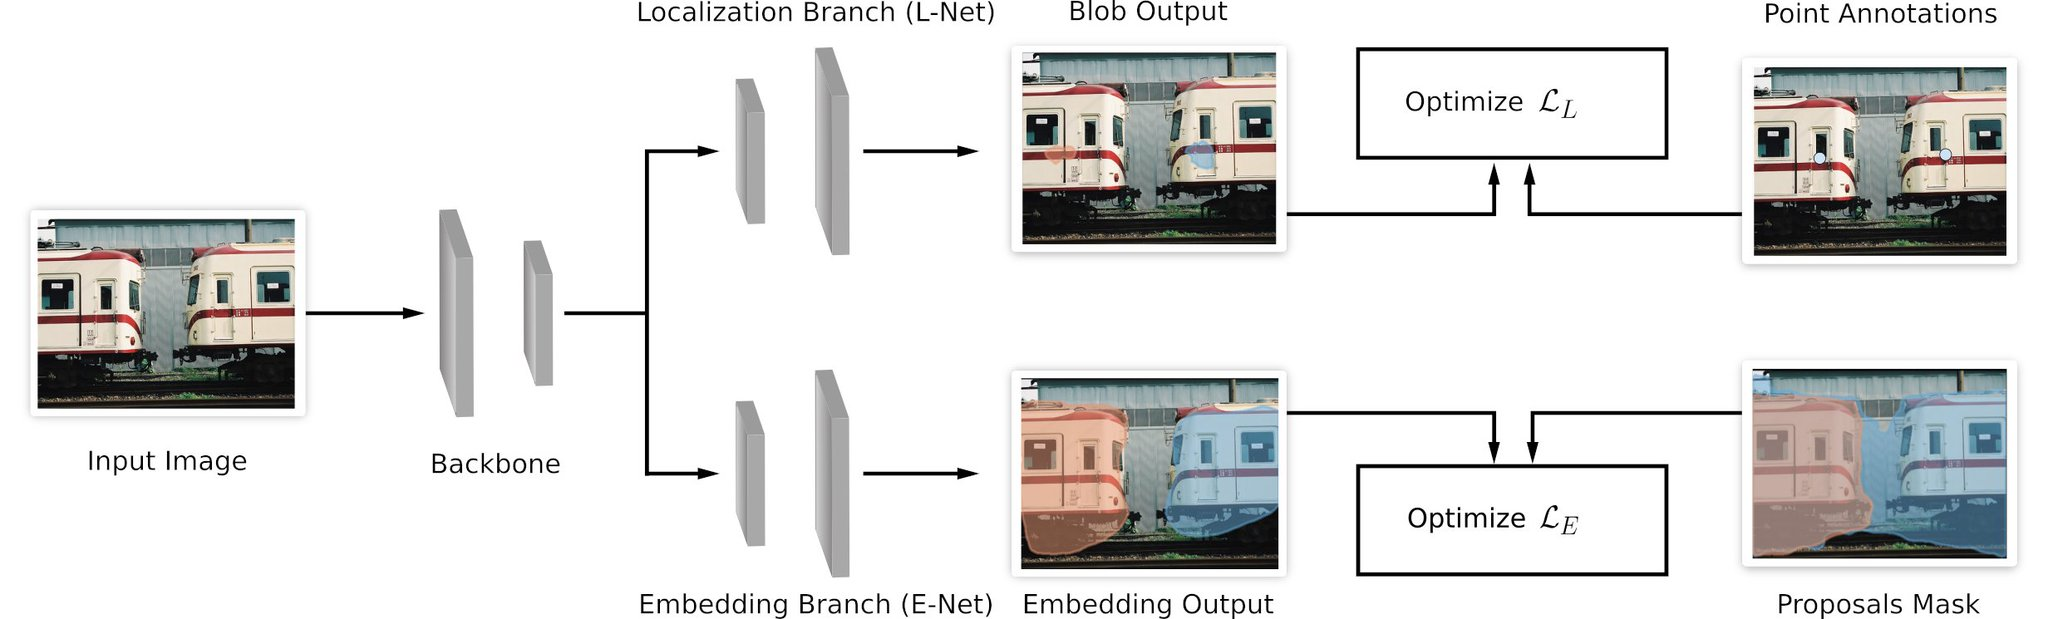
\includegraphics[width=10cm]{/home/thesis/images/Laradji_WISE.jpeg}
    \caption{Illustration from \cite{Laradji2020}. The WISE approach consists of two branches: The Embedding branch and the Localization branch.}
    \label{fig:Laradji_WISE}
\end{SCfigure}
\par{
    The WISE model seems to perform well on the PASCAL VOC 2012 dataset, the Cityscapes dataset and the COCO 2014 dataset. 
    Nevertheless, the author abandoned it in \cite{Laradji2021,Laradji2020b}, where he demonstrated a weakly supervised network to segment patient lungs and zones of opacity and consolidation in the lungs of potential \Gls{covid} patients.
    There are several potential reasons for this. 
    Two of those seem essential for this work. 
    First, the WISE approach seems to assume the expert positions the annotation point right in the centre of each object instance.
    Second, the approach is complex, and the double branch inference is computation and memory intensive. 
    This project assumes that experts can provide different point labels for the same instance at random locations in the instance.
    Since volume data is is more memory intensive than picture data, it is beneficial to avoid overly complex and memory-intensive approaches.
}
\par{
    In \cite{Laradji2021}, Laradji et al. introduces an approach based on the consistency loss, combined with binary cross-entropy.
    This approach, illustrated in figure \ref{fig:Laradji_consistency} is used and extended in this project.
    Details are provided starting on page \pageref{sec:model_concept}.
}
\begin{SCfigure}[][htb]
    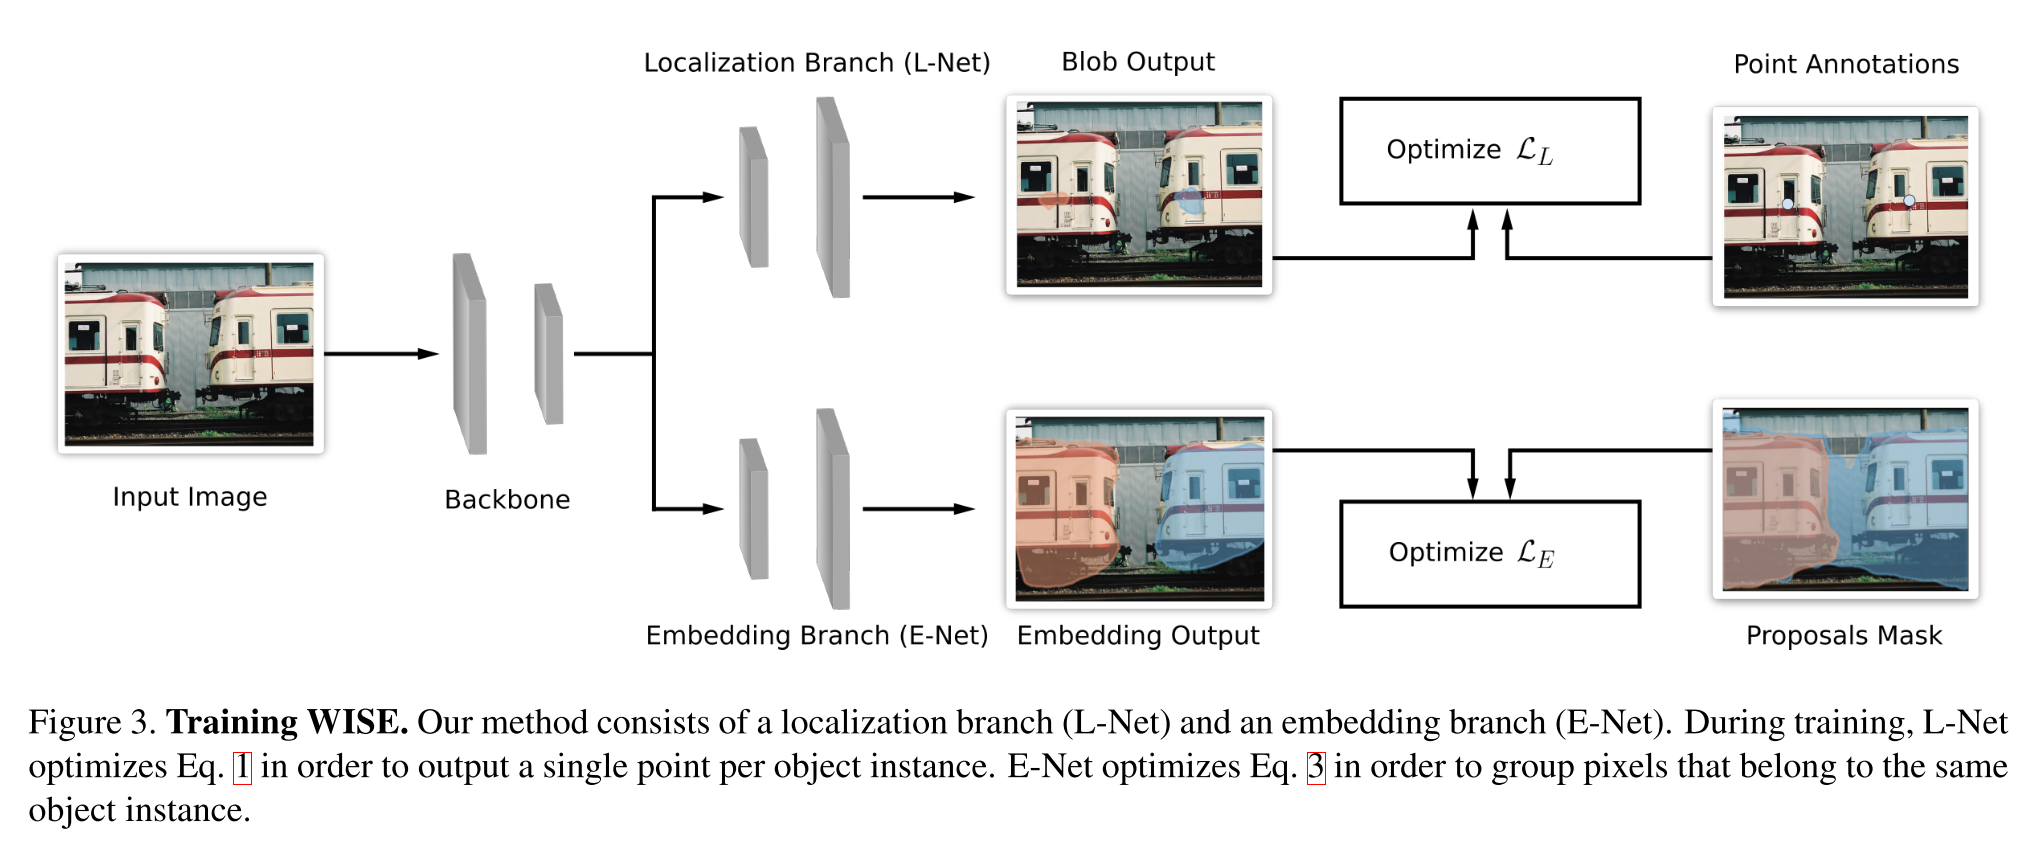
\includegraphics[width=10cm]{/home/thesis/images/Laradji_architecture.png}
    \caption{Illustration from \cite{Laradji2021}. The consistency loss approach is based on the combination of two loss terms: the \Gls{unsupervisedl} consistency loss and the (weakly) \Gls{supervisedl} point (cross entropy) loss.}
    \label{fig:Laradji_consistency}
\end{SCfigure}
\par{
    Figure \ref{fig:Laradji_consistency} illustrates the basic concept of the consistency model.
    The network output is required to be consistent under a geometric transformation, i.e. the network output when presented with image $\mathcal{X}_i$ rotated over $90^\circ$ should be the rotation of the network output when presented with image $\mathcal{X}_i$.
}